% Ta đã học 4 mô hình, hãy viết một tài liệu mô tả chi tiết 
% từng mô hình sao cho người chưa biết gì cũng có thể hiểu được
% Là gì, vẽ hình minh họa, phân tích ưu nhược điểm
% giải thích tại sao có ưu nhược điểm đấy
% khi nào sử dụng
% Chỉ có mô hình chữ V cần dùng mô tả của thác nước and nói
% rõ sự khác biệt
\documentclass[14pt]{extarticle}
\usepackage{multicol}
\usepackage[utf8]{vietnam}
\usepackage[left = 2cm, right = 2cm]{geometry}
\usepackage{amsmath}
\usepackage{amsfonts}
\usepackage{amssymb}
\usepackage{mathtools}
\usepackage{changepage}
\usepackage{graphicx}
\title{\textbf{MÔ HÌNH PHÁT TRIỂN PHẦN MỀM CƠ BẢN}}
\author{\textbf{Nguyễn Minh Hiển}}


\begin{document}
\newpage
\maketitle
\tableofcontents
\newpage
\section*{Giới thiệu mô hình phát triển phần mềm}
\addcontentsline{toc}{section}{Giới thiệu mô hình phát triển phần mềm}

Đầu tiên, mô hình là mô phỏng lại một quy trình nào đó đã được thực hiện thành công
trong thực tế để có thể áp dụng vào các quy trình khác.\\
Ví dụ: Mô hình xóa đói giảm nghèo. Khi các công việc, cách làm xóa đói
giảm nghèo đã được thực hiện thành công ở một nơi nào đó, thì chính quyền
có thể khái quát nó thành một mô hình để áp dụng vào các nơi khác mà có
những điều kiện về tự nhiên, về xã hội tương đồng.\\

Thứ hai, vòng đời của một phần mềm bao gồm hai giai đoạn:
\begin{itemize}
  \item Giai đoạn phát triển phần mềm: bao gồm cái hoạt động:
        \begin{itemize}
          \item Phân tích và đặc tả yêu cầu
          \item Thiết kế
          \item Implementing và kiểm thử đơn vị
          \item Kiểm thử
        \end{itemize}
  \item Giai đoạn vận hành và bảo trì
\end{itemize}

Như vậy, mô hình phát triển phần mềm là khái quát lại một quy trình phát triển
phần mềm có hiệu quả được đúc rút từ kinh nghiệm thực tế. Mô hình
này bao gồm các pha, các nguyên tắc, nguyên lý để hướng
đến mục tiêu cuối cùng là phát triển phần mềm một cách hiệu
quả nhất.\\

Mỗi mô hình phát triển phần mềm đều có những ưu nhược điểm
riêng, và phù hợp với các dự án có một số đặc điểm nhất định.
Do đó, việc lựa chọn mô hình phát triển phần mềm phù hợp với
dự án là một vấn đề quyết định đến thành công của dự án.
\newpage
\section{Mô hình thác nước (Waterfall model)} \label{sec:waterfall}

\subsection{Định nghĩa}
Mô hình thác nước là mô hình phát triển phần mềm đầu tiên,
sơ khai nhất, tự nhiên nhất và vẫn còn phổ biến đến hiện nay.

Mô hình này chia quá trình phát triển phần mềm thành các giai đoạn
tuần tự (các pha), nghĩa là hoàn thành pha này mới tài liệu để
chuyển sang được pha tiếp theo.
Điều này khá giống với dòng thác nước, nước đổ từ bậc trên
xuống bậc dưới vậy, bậc trên phải đầy thì nước mới tràn xuống bậc dưới.

Từ vòng đời của một phần mềm, mô hình thác nước được xây dựng như sau:
\begin{figure}[h]
  \centering
  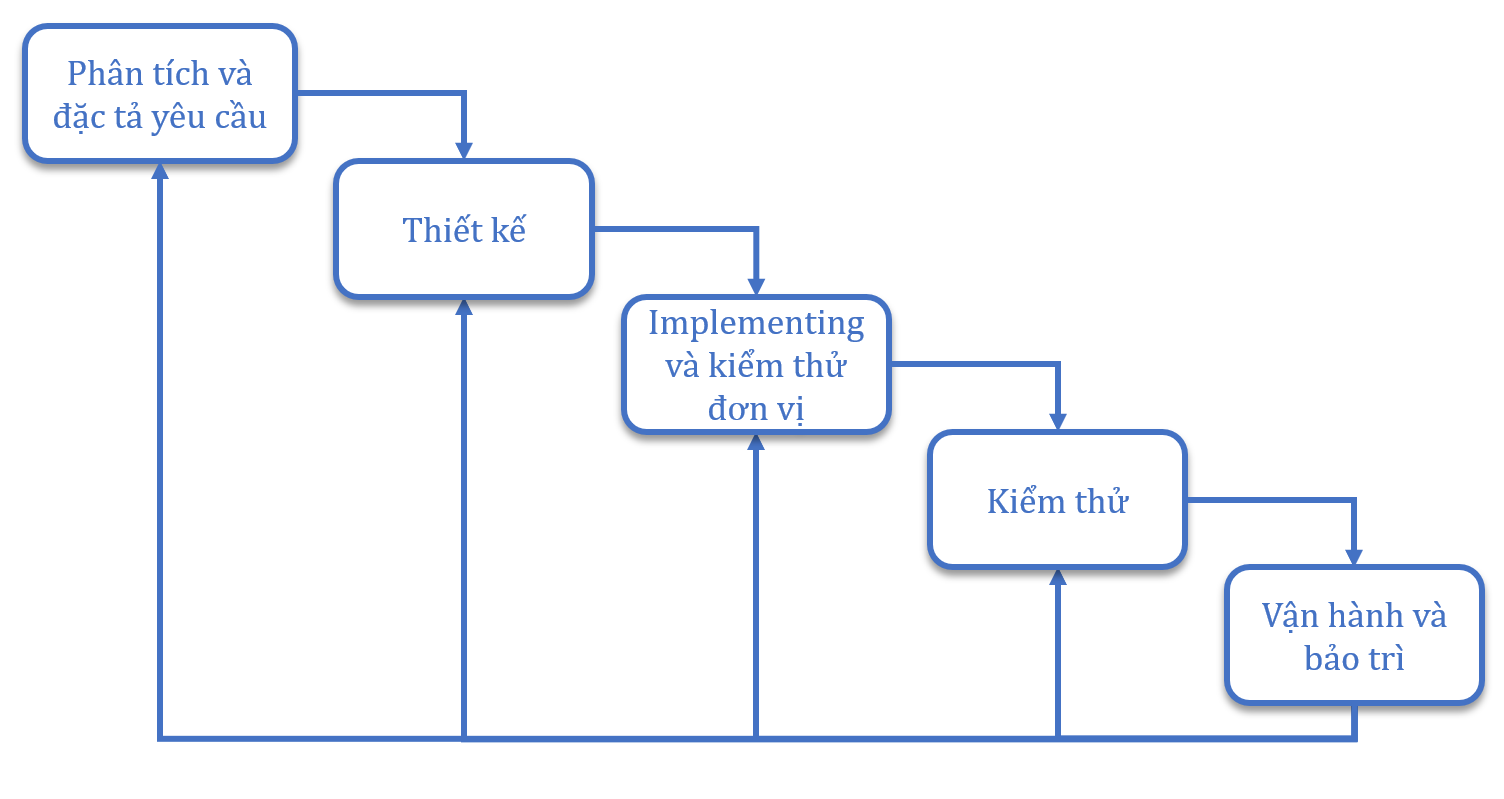
\includegraphics[width=\textwidth]{waterfall2.png}
  \caption{Mô hình thác nước}
  \label{fig:waterfall}
\end{figure}

Tuy nhiên, không phải pha nào cũng có thể thực hiện một cách hoàn hảo.
Lỗi có thể xảy ra ở bất kỳ pha nào, tại bất kỳ thời điểm nào, và giả
sử lỗi được phát hiện là của pha trước đó thì ta cần phải quay lại pha
trước đó để sửa. Một điều cần chú ý là để đảm bảo tính tuần tự của
mô hình thác nước, khi gặp lỗi, ta phải dừng pha đang làm lại (nói
cách khác là dừng cả quy trình lại), lật lại pha trước đó để xem
vấn đề ở đâu và sửa lỗi. Điều này có thể gây đến nhiều hệ lụy sẽ được
đề cập ở phần nhược điểm bên dưới.

\subsection{Ưu điểm}

\subsubsection*{Dễ hiểu, dễ học}
Có thể thấy, mô hình thác nước là mô hình cơ bản nhất: chỉ là việc
triển khai tuần tự các hoạt động trong vòng đời phát triển của một phần mềm thành
các pha.
Việc triển khai tuần tự nghĩa là các hoạt động được thực hiện một cách rõ ràng,
lần lượt, không có sự chồng chéo giữa các hoạt động. Điều này giúp cho việc
hiểu và học mô hình này trở nên dễ dàng hơn.

\subsubsection*{Đảm bảo được phần mềm có chất lượng cao}
Khi đã xác định sử dụng mô hình thác nước để phát triển phần mềm
thì người ta cũng xác định việc triển khai tuần tự các pha. Nhận thức
được điều đó, họ luôn phải cẩn thận trong từng bước bởi rất ít cơ hội
để quay lại và sửa lỗi. Mỗi lần làm cần kiểm tra lại, cần có tài liệu
đầy đủ. Và mỗi pha cũng cần làm sao cho việc quay lại và sửa lỗi
tốn ít thời gian và kinh phí nhất có thể.\\

\subsubsection*{Dễ quản lý}
Quy trình phát triển phần mềm theo mô hình thác nước dễ quản lý do
việc triển khai theo từng pha nên dễ quản lý tiến độ. Pha sau cũng luôn
có cái nhìn tổng thể về hệ thống của các pha trước nên mô hình thác nước
sẽ có chất lượng cao hơn các mô hình làm từng phần.

\subsection{Nhược điểm}

\subsubsection*{Chỉ phù hợp với dự án vừa và nhỏ}
Vấn đề này sẽ được phân tích ở bên dưới

\subsubsection*{Chi phí cao và thời gian lâu}
Về chi phí cao, do việc triển khai tuần tự và làm cẩn thận từng pha
để phần mềm đầu ra có chất lượng cao nên chi phí sẽ tăng lên.


Về thời gian, do việc triển khai tuần tự nên mỗi thời điểm chỉ có một
pha được thực hiện nên thời gian sẽ kéo dài hơn so với các mô hình khác.

Chưa kể nếu có lỗi xảy ra ở pha nào đó, việc dừng quy trình để quay lại
pha trước đó sẽ làm tăng thêm thời gian và chi phí.

\subsubsection*{Không linh hoạt, nếu phát hiện lỗi ở những bước cuối là thảm họa}

Do việc triển khai tuần tự nên nếu có lỗi xảy ra ở pha nào đó, cần
dừng quy trình để quay lại pha trước đó, từ đó làm tăng thời gian và chi phí
để chỉnh sửa. Điều này thật sự không linh hoạt nếu khách hàng thường xuyên
thay đổi yêu cầu.

Giả sử lỗi bắt nguồn từ những pha đầu tiên thì ta cần rất nhiều thời gian,
chi phí để rework lại các bước trước.
Hệ quả là chúng ta có thể hết thời gian giao phần mềm cho khách hàng, hoặc
hết kinh phí để hoàn thành dự án.

\subsubsection*{Tất cả các yêu cầu phải rõ ràng} \label{sec:clear-req}

Ví dụ về một yêu cầu không rõ ràng: Khách hàng yêu cầu một phần mềm hiệu quả.
Nhưng người ta vẫn chưa biết nó là cái gì, nó làm được những gì, nó dùng
như thế nào.

Khi khách hàng có yêu cầu về phần mềm chưa rõ ràng (dù chỉ là một trong
nhiều yêu cầu), thì ta không thể sử dụng mô hình thác nước bởi yêu cầu đó
sẽ khiến ta phải dừng pha đặc tả yêu cầu lại cho đến khi yêu cầu rõ ràng.\\


\subsubsection*{Kiểm thử muộn và chung chung}
Kiểm thử bao gồm có $4$ mức: kiểm thử đơn vị, kiểm thử tích hợp, kiểm thử
hệ thống và kiểm thử chấp nhận. Việc kiểm thử chỉ thực hiện khi có sản phẩm
hay một phần sản phẩm cuối cùng.

Có thể thấy trong mô hình thác nước, lần đầu tiên khách hàng nhìn thấy sản phẩm
(ở bước kiểm thử chấp nhận) cũng là thời điểm họ sử dụng phần mềm luôn.

Một nguyên tắc cơ bản của phát triển phần mềm là cố gắng đưa người dùng vào
test sớm nhất có thể. Tuy nhiên, với đặc điểm trên thì mô hình thác nước
không thể triển khai được nguyên tắc này. Điều đó có thể dẫn đến các
hệ lụy sau:
\begin{itemize}
  \item Nếu phần mềm chưa đáp ứng được yêu cầu của khách hàng hay
        UI/UX không tốt, thì ta sẽ không kịp sửa cho khách hàng được.
  \item Thời gian đào tạo người dùng ngắn.\\
        Khi phát triển phần mềm, có nhiều lỗi phát sinh là do khách hàng
        không biết cách sử dụng phần mềm, chứ không phải do lỗi của phần mềm.
        Do đó, ta cần đào tạo khách hàng để họ có thể dùng thạo phần mềm.
        Mức hài lòng của khách hàng cũng phụ thuộc rất nhiều vào việc họ
        có thể sử dụng phần mềm một cách thành thạo hay không.\\
        Tuy nhiên, trong mô hình thác nước, lần đầu nhìn thấy sản phẩm cũng
        là lúc khách hàng phải học cách sử dụng nó luôn nên họ rất dễ vấp
        khi dùng. Điều này khó hơn hẳn với việc họ được liên tục hỏi ý kiến
        hay nhìn thấy, dùng thử phần mềm trước đó.
\end{itemize}

\subsection{Khi nào sử dụng}
Mô hình thác nước chỉ phù hợp với các dự án vừa và nhỏ, yêu cầu rõ ràng.

Nó không phù hợp với các dự án lớn bởi rủi ro cao, nên nếu sử dụng chỉ làm tăng
chi phí, thời gian bởi nếu có lỗi xảy ra ở pha nào đó, ta cần dừng quy trình để
quay lại pha trước sửa lỗi. Tương tự, nó cũng không phù hợp với các dự án mà
yêu cầu thay đổi thường xuyên.

Với yêu cầu không rõ ràng, mô hình thác nước cũng không phù hợp vì ta phải
dừng lại ở pha đặc tả yêu cầu cho đến khi yêu cầu rõ ràng.



\newpage
\section{Mô hình chữ V (V model)}
\subsection{Định nghĩa}
Mô hình chữ V là mô hình phát triển phần mềm được cải tiến từ
mô hình thác nước. Về cơ bản, mô hình chữ V cũng triển khai tuần tự
các pha như mô hình thác nước.
\begin{figure}[h]
  \centering
  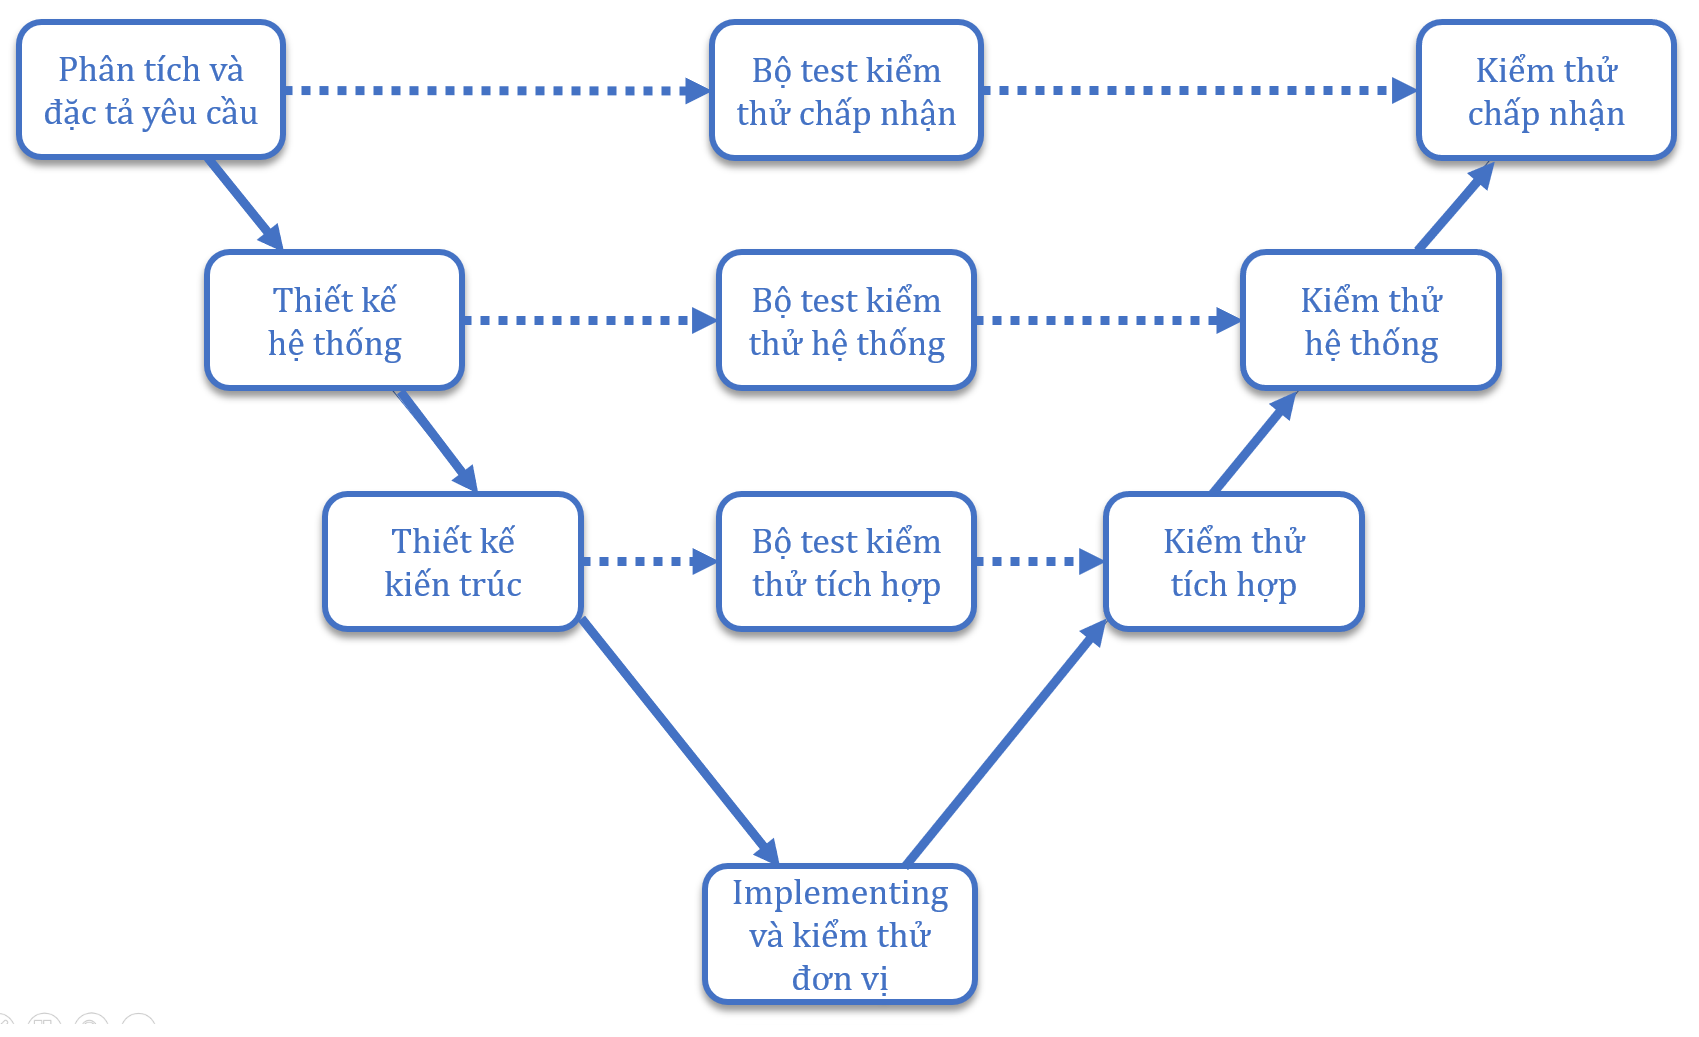
\includegraphics[width=\textwidth]{v-model.png}
  \caption{Mô hình chữ V}
  \label{fig:v-model}
\end{figure}

Tuy nhiên, mô hình chữ V cải tiến
từ mô hình thác nước ở hai điểm sau:
\begin{itemize}
  \item \textbf{Đẩy việc sinh test lên sớm hơn}\\
        Trong mô hình thác nước, kiểm thử chỉ thực hiện sau pha \textit{implementing
          và kiểm thử đơn vị}. Nói chính xác hơn là sau pha này mới thực hiện
        việc sinh test và kiểm thử. Đầu ra của các pha \textit{phân tích và đặc tả
          yêu cầu}, \textit{thiết kế} chỉ có tài liệu cho các pha sau. \\
        Trong mô hình chữ V, người ta đẩy việc sinh test lên sớm hơn. Ví dụ,
        với pha \textit{phân tích và đặc tả yêu cầu}, đầu ra sẽ có thêm các bộ test
        cho pha đó. Sau này khi có sản phẩm hoàn chỉnh để kiểm thử, chỉ
        cần qua được các bộ test này là sản phẩm đáp ứng được đặc tả yêu cầu.
        Tương tự với pha \textit{thiết kế}.

  \item \textbf{Phân chia kiểm thử thành nhiều mức}\\
        Trong mô hình thác nước, việc kiểm thử vẫn còn quá chung chung.\\
        Trong mô hình chữ V, người ta phân chia kiểm thử thành nhiều mức:
        \begin{itemize}
          \item Kiểm thử đơn vị
          \item Kiểm thử tích hợp
          \item Kiểm thử hệ thống
          \item Kiểm thử chấp nhận
        \end{itemize}

\end{itemize}

\subsection{Ưu điểm}
Mô hình chữ V vẫn thừa kế được những ưu điểm của mô hình thác nước:
\begin{itemize}
  \item Dễ hiểu, dễ học. Tuy có chút thay đổi, nhưng mô hình chữ V vẫn
        giữ nguyên cấu trúc tuần tự của mô hình thác nước nên vẫn dễ hiểu, dễ học.

  \item Đảm bảo được phần mềm có chất lượng cao
  \item Dễ quản lý tiến độ
\end{itemize}
Tuy nhiên, mô hình chữ V còn có những ưu điểm riêng:
\subsubsection*{Phân chia kiểm thử thành nhiều mức}
Phân chia kiểm thử thành nhiều mức giúp cho việc kiểm thử trở nên chặt chẽ,
chi tiết hơn.
\subsubsection*{Đẩy việc sinh test lên sớm hơn}
Đẩy việc sinh test lên sớm hơn giúp cho các test cases tốt hơn, sát hơn với
yêu cầu của khách hàng, với thiết kế của phần mềm.\\
Sau này chỉ cần qua được các test cases này là sản phẩm đáp ứng được yêu cầu hay
thiết kế.\\
\subsection{Nhược điểm}
Do chỉ cải tiến về phần kiểm thử của mô hình thác nước nên mô hình chữ V
vẫn còn những nhược điểm của mô hình thác nước:
\begin{itemize}
\item {Không linh hoạt, chỉ phù hợp với dự án vừa và nhỏ}
\item{Chi phí cao và thời gian lâu}
\item{Phát hiện lỗi ở những bước cuối là thảm họa}
\item{Tất cả các yêu cầu phải rõ ràng}
\end {itemize}
\subsection{Khi nào sử dụng}
Tương tự với mô hình thác nước, mô hình chữ V chỉ phù hợp với các dự án vừa và nhỏ,
yêu cầu rõ ràng.\\

Hiện nay, khi nhắc đến mô hình thác nước, chúng ta thường sử dụng mô hình chữ V
thay cho mô hình thác nước nguyên thủy ở Mục ~\ref{sec:waterfall}.

\newpage
\section{Mô hình bản mẫu (Prototype model)}
\subsection{Định nghĩa}
Mô hình bản mẫu là mô hình phát triển phần mềm được xây dựng
dựa trên việc tạo ra các bản mẫu (prototype) của phần mềm cho người dùng
sử dụng thử.\\

\begin{figure}[h]
  \centering
  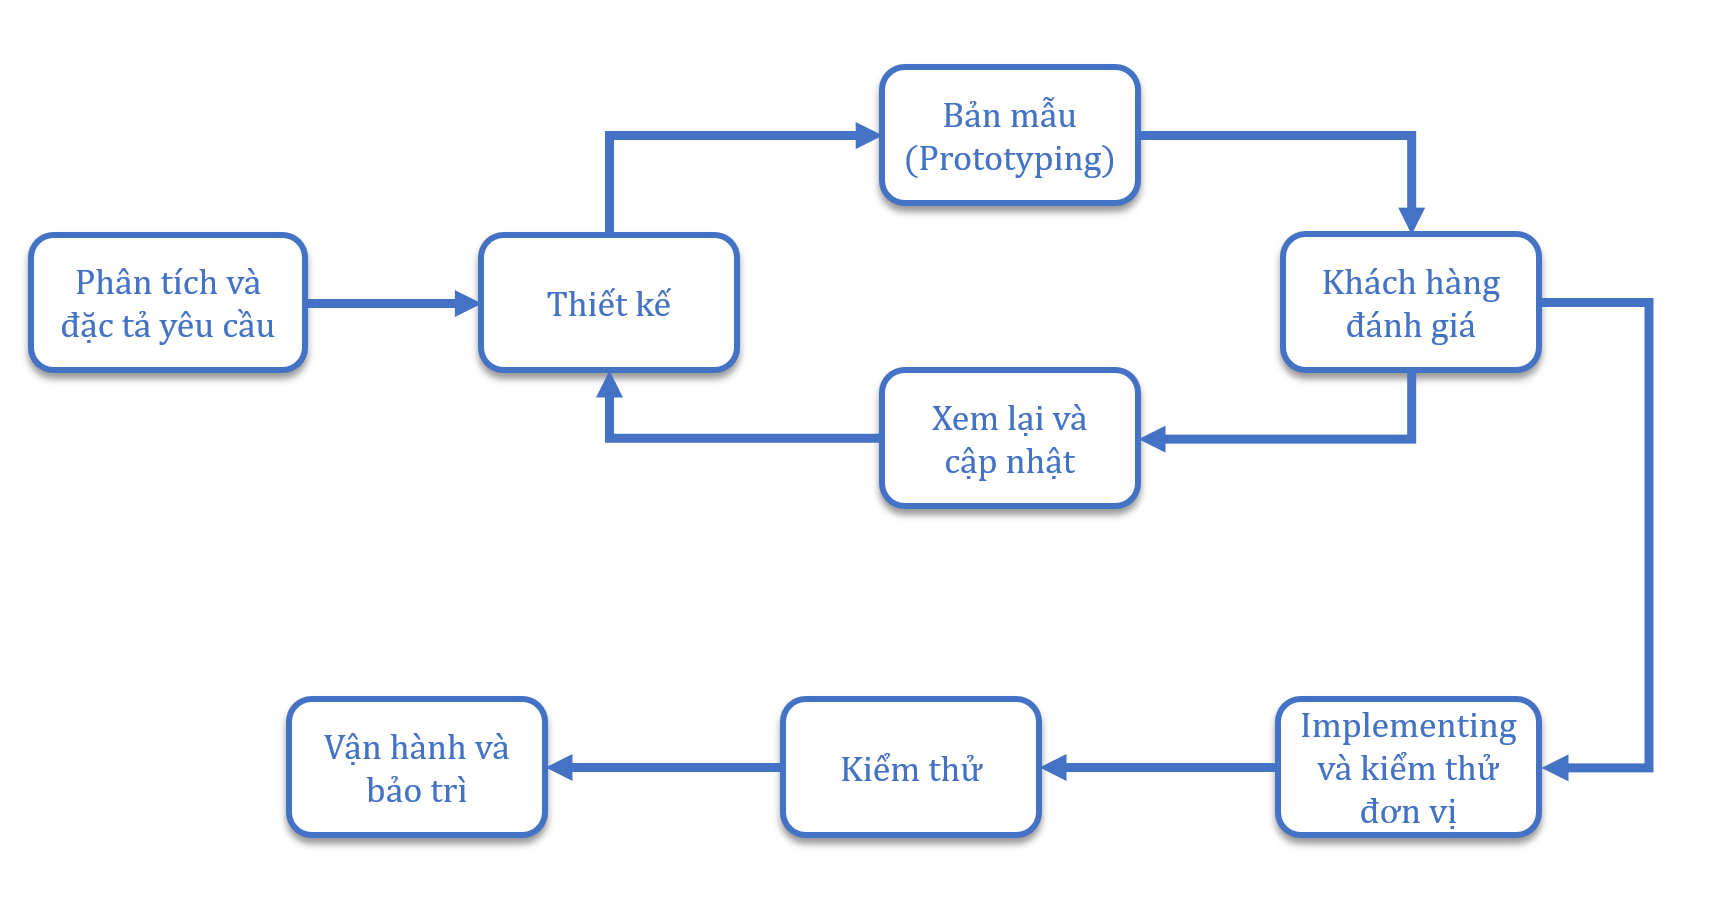
\includegraphics[width=\textwidth]{prototype.png}
  \caption{Mô hình bản mẫu}
  \label{fig:prototype-model}
\end{figure}

Khi khách hàng có yêu cầu về phần mềm chưa rõ ràng (dù chỉ là một trong
nhiều yêu cầu), thì ta không thể sử dụng mô hình thác nước (Xem phần ~\ref{sec:clear-req}).\\

Để giải quyết vấn đề này, mô hình bản mẫu sẽ liên tục thiết kế các bản mẫu
(một giao diện giả của phần mềm) để cho khách hàng xem và đánh giá cho
đến khi họ có thể đưa ra yêu cầu rõ ràng để ta có thể triển khai các pha
tiếp theo.

\subsection{Ưu điểm}
\subsubsection*{Giải quyết yêu cầu không rõ ràng}
Mô hình bản mẫu giải quyết yêu cầu không rõ ràng của khách hàng
bằng cách trực quan hóa yêu cầu bằng bản mẫu (một giao diện giả)
để khách hàng có thể xem và đưa ra yêu cầu chính xác hơn.
Cách này rất hữu dụng khi khách hàng không biết chính xác họ muốn
cái gì, họ muốn cái gì nhưng không biết nó như thế nào.

\subsection{Nhược điểm}
\subsubsection*{Thời gian và chi phí cho bản mẫu lớn}
Chúng ta không thể biết được bao nhiêu bản mẫu cần thiết cho một phần mềm (do
điều này phụ thuộc vào ý kiến của khách hàng) nên thời gian cho bản mẫu
có thể kéo dài.\\
Do thời gian cho bản mẫu nhiều nên thời gian và chi phí cho việc thiết kế,
implementing, và kiểm thử ít hơn. Hậu quả là chất lượng có vấn đề, tài liệu
có thể không đầy đủ.

\subsection{Khi nào sử dụng}
Ý tưởng của mô hình thiết kế rất hay tuy nhiên lại không được sử dụng phổ biến
vì thời gian và chi phí cho bản mẫu quá lớn.
Vì thế, mô hình bản mẫu thường được sử dụng trong các dự án vừa và nhỏ.\\

Trong thực tế người ta thường dùng ý tưởng bản mẫu như một cách để thu thập
yêu cầu của khách hàng.

\newpage
\section{Mô hình xoắn ốc (Spiral model)}
\subsection{Định nghĩa}

Mô hình xoắn ốc là sự kết hợp của mô hình thác nước, mô hình bản mẫu
và phân tích rủi ro, được phát triển theo cách tăng dần (incremental).\\

\begin{figure}[h]
  \centering
  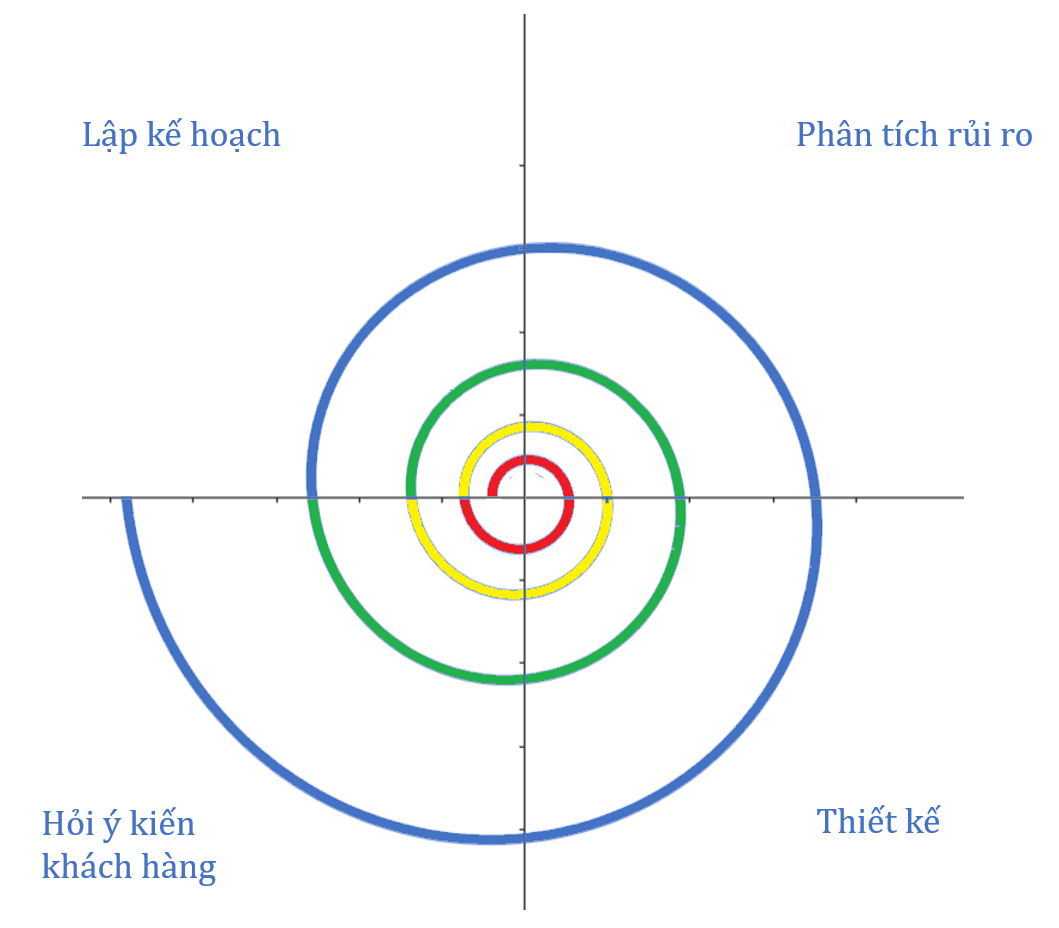
\includegraphics[width=0.7\textwidth]{spiral.png}
  \caption{Mô hình xoắn ốc}
  \label{fig:spiral-model}
\end{figure}

Mỗi pha cũng chính là mỗi vòng xoáy bắt đầu bằng việc lập kế hoạch
và kết thúc bằng hỏi ý kiến khách hàng. Sau khi kết thúc một vòng xoáy,
có thể tiếp tục ở một level cao hơn (vòng xoáy tiếp theo) hoặc dừng lại.\\
Ý tưởng chính của mô hình này là chia để trị. Chúng ta sẽ làm các tính
năng cốt lõi (core) trước, sau mới đến các tính năng ở mức trung bình
(medium level), cuối cùng là các tính năng ít sử dụng.\\

Mỗi pha là một vòng xoáy, và mỗi vòng xoáy sẽ có các việc sau:
\begin{itemize}
  \item \textbf{Lập kế hoạch}\\
        Lập kế hoạch cho vòng xoáy này, xác định các mục tiêu, rủi ro,
        chi phí, thời gian, nguồn lực cần thiết.
  \item \textbf{Phân tích rủi ro}\\
        Phân tích rủi ro cho vòng xoáy này, xác định các rủi ro có thể
        xảy ra và cách xử lý nó.\\
        Trước tiên cần dự đoán rủi ro: những rủi ro nào có thể
        xảy ra, xác suất xảy ra là bao nhiêu, hệ quả của các rủi ro?
        Nếu chấp nhận rủi ro để làm tiếp thì cần đưa ra giải pháp phòng chống
        như thế nào?\\
        Đây và vấn đề phức tạp, cần có chuyên gia rất thâm niên trong quản lý
        dự án.

  \item \textbf{Phát triển phần mềm}\\
        Một phần mô hình thác nước được sử dụng ở đây với các pha tuần tự:
        \begin{itemize}
          \item Phân tích và đặc tả yêu cầu
          \item Thiết kế
          \item Implementing và kiểm thử đơn vị
          \item Kiểm thử
        \end{itemize}

  \item \textbf{Hỏi ý kiến khách hàng}\\
        Hỏi ý kiến khách hàng về sản phẩm để chỉnh sửa hay thêm
        tính năng ở các vòng xoáy sau này.
\end{itemize}

\subsection{Ưu điểm}
\subsubsection*{Có thể thêm tính năng hay chỉnh sửa ở các pha sau (Tính linh hoạt)}
Mô hình xoắn ốc được thiết kế để có thể thêm tính năng hay chỉnh sửa ở
các vòng xoắn tiếp theo dựa trên phản hồi ở pha trước. Thêm vào đó,
bằng cách phân tích và hạn chế các rủi ro, mô hình có thể quản lý những
thay đổi, bổ sung phát sinh dễ dàng hơn.
\subsubsection*{Dễ dàng ước chừng chi phí hơn}
Mô hình xoắn ốc luôn có bước lên kế hoạch và phân tích và hạn chế rủi ro
ở từng vòng xoắn, cùng với tính linh hoạt giúp tiết kiệm được chi phí. Ở từng
vòng xoắn cũng có nhận phản hồi từ khách hàng để tinh chỉnh lại chi phí cho phù
hợp.
\subsubsection*{Các tính năng được thêm vào một cách có hệ thống}
Không phải ngẫu nhiên các tính năng được chọn phát triển ở vòng xoắn trước hay sau.
Chúng ta sẽ làm các tính năng cốt lõi (core) trước, sau mới đến các tính năng ở
mức trung bình (medium level), cuối cùng là các tính năng ít sử dụng.\\
Như vậy, khách hàng cũng sẽ sớm trải nghiệm và đánh giá các tính năng cốt lõi
họ cần để có thể chỉnh sửa nếu cần.
\subsubsection*{Kết thúc từng pha bằng hỏi ý kiến khách hàng}
Điều này có thể trực quan hóa cho khách hàng thấy được sự tiến triển của dự án
và có thể đưa ra ý kiến sớm nhất có thể.

\subsection{Nhược điểm}
\subsubsection*{Nguy cơ vượt quá ngân sách hay chậm tiến độ}
Mỗi vòng lặp thì lại có thêm các tính năng được chỉnh sửa hay bổ sung
có thể dẫn đến dự án vượt khỏi ngân sách, kế hoạch ban đầu.\\
Việc đánh giá rủi ro yêu cầu sự chuyên môn cao, và nếu không đánh giá
chính xác thì có thể dẫn đến việc dự án vượt quá ngân sách, chậm tiến độ.
\subsubsection*{Chỉ phù hợp với các dự án lớn}
Được phân tích ở phần bên dưới
\subsection{Khi nào sử dụng}
Mô hình xoắn ốc thường sử dụng cho các hệ thống lớn, yêu cầu nhiều thay đổi.
Các hệ thống càng lớn thì rủi ro cao dẫn đến chi phí cho rủi ro lớn, ko còn
chi phí phát triển, software fail. Cần phải có chuyên gia về rủi ro, quản lý dự án
thâm niên mới có thể dự đoán và hạn chế rủi ro.\\
Do đó, mô hình xoắn ốc không sử dụng cho các hệ thống vừa và nhỏ bởi rủi ro ít,
nên nếu sử dụng chỉ làm tăng chi phí, thời gian.


\end{document}